Symmetry elements in a crystal and the corresponding extinction conditions.
If you are comfortable with spotting them under exam conditions then this question can be quite straightforward to solve.%
\footnote{That being said, CuO is a monoclinic crystal with space group C2/c. \url{http://pd.chem.ucl.ac.uk/pdnn/symm3/centred.htm} is an excellent webpage describing it. Apologies if I have missed any symmetry elements in the answer!}

\begin{parts}
	\part Sketch of the crystal:
	\begin{figure}[H]
		\centering
		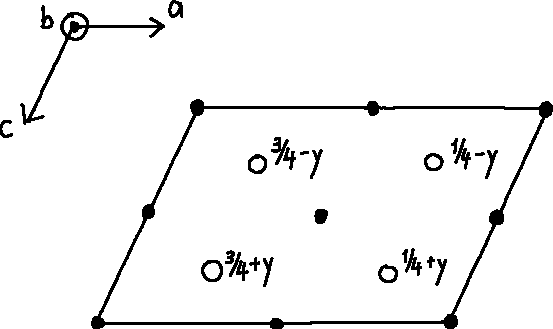
\includegraphics[width=.7\linewidth]{q1-crystal}
	\end{figure}
	\begin{subparts}
		\subpart Inversion points exist at $\rbracket{\diagfrac{1}{2}, \diagfrac{1}{2}, \diagfrac{1}{2}}$ and all Cu atoms.
		
		\subpart There exists no mirror plane.
		
		\subpart We see that there are $2_b$ about the O atoms. In $ac$ coordinates, they are $(\diagfrac{1}{4}, \diagfrac{1}{4})$, $(\diagfrac{1}{4}, \diagfrac{3}{4})$, $(\diagfrac{3}{4}, \diagfrac{1}{4})$, and $(\diagfrac{3}{4}, \diagfrac{3}{4})$.
		
		\subpart A diagonal n-glide plane at $b=\diagfrac{1}{4}$.
	\end{subparts}
	
	\part From the diagram above, we see that the basis of 2 O's and 1 Cu may be replicated via the translation $a = \diagfrac{1}{2}$, $b = \diagfrac{1}{2}$ $\Rightarrow$ C centering.
	
	\part We know that structure factor $S_{hkl} = S_\textnormal{lattice} \times S_\textnormal{basis}$.
	
	From the C-centering, we have $S_\textnormal{lattice} \propto \rbracket{1 + \mathrm{e}^{2\pi i\rbracket{h/2 + k/2}}}$.
	Thus we have $h+k=$ odd for extinction.
	
	We also have the following symmetry equivalent positions due to the glide: $x, y, z \xrightarrow{\textnormal{glide}} \diagfrac{1}{2}+x, \diagfrac{1}{2}-y, \diagfrac{1}{2}+z$.
	
	So the structure factor will always have a common factor of:
	\begin{equation*}
		\sbracket{
		 \mathrm{e}^{2\pi i\rbracket{hx+ky+lz}} + \mathrm{e}^{2\pi i\rbracket{h(1/2 + x) + k(1/2 - y) +l(1/2 + z)}}
		}
		= \mathrm{e}^{2\pi i\rbracket{hx+ky+lz}}
		\sbracket{
		 1 + \mathrm{e}^{\pi i\rbracket{h+l+k-4ky}}
		}
	\end{equation*}
	Thus another extinction condition is $k=0$ and $h+l=$ odd.%
	\footnote{This webpage from UCL is fantastic on summarising glide-derived \textit{reflection} conditions: \url{http://pd.chem.ucl.ac.uk/pdnn/symm4/glide.htm}}
\end{parts}